\documentclass[11pt]{article}
\usepackage[utf8]{inputenc}
\usepackage[T1]{fontenc}
\usepackage{amsmath}
\usepackage{amssymb}
\usepackage{multicol}
\usepackage{geometry}
\usepackage{tikz}
\usepackage{enumitem}
\usepackage{xcolor}
\usepackage{titlesec}
\usetikzlibrary{shadows}
\usepackage{graphicx}
\usepackage{ragged2e} % Para texto justificado

% Configurações de layout
\geometry{a4paper, left=1cm, right=1cm, top=0.5cm, bottom=1.2cm}
\setlength{\columnseprule}{0.4pt}

% Cores para títulos
\titleformat{\section}{\normalfont\Large\bfseries\color{blue}}{\thesection}{1em}{}
\titleformat{\subsection}{\normalfont\large\bfseries\color{red}}{\thesubsection}{1em}{}

\title{\textcolor{blue}{Cultura Digital \\ Cibersegurança: Proteção no Mundo Digital}}
\author{Professor: Jefferson}
\date{}

\begin{document}

\maketitle
\vspace{-1cm}

\begin{center}
\large{Nome: \underline{\hspace{8cm}} \quad Turma: \underline{\hspace{3cm}}}
\end{center}

\begin{multicols}{2}

\section*{Objetivo da Aula}

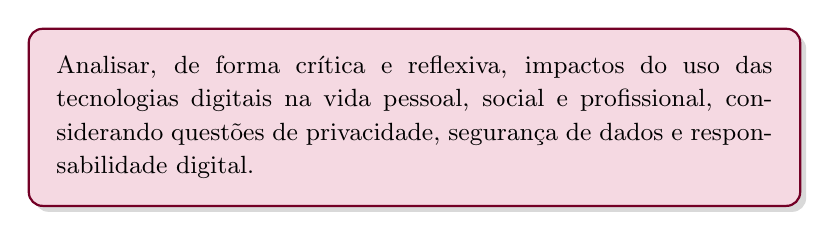
\begin{tikzpicture}
\node[rectangle, 
      fill=purple!15, 
      rounded corners=5pt, 
      inner sep=10pt, 
      draw=purple!60!black, 
      thick,
      drop shadow={opacity=0.3},
      text width=0.75\linewidth,
      align=justify] 
{
\small
 Analisar, de forma crítica e reflexiva, impactos do uso das tecnologias digitais na vida pessoal, social e profissional, considerando questões de privacidade, segurança de dados e responsabilidade digital.
};
\end{tikzpicture}

\vspace{5mm}

\section*{1. Introdução: Cibersegurança e Reputação Digital}

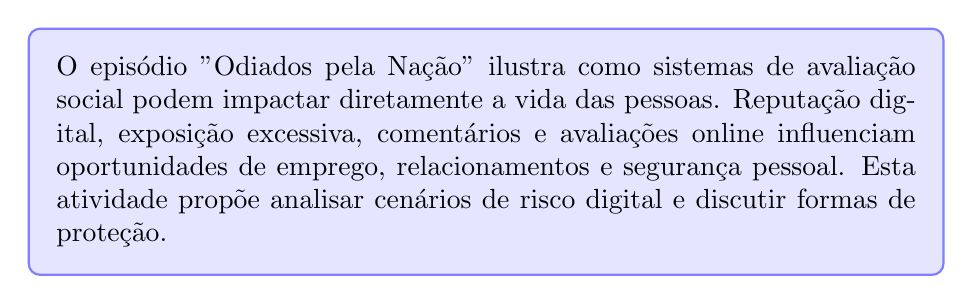
\begin{tikzpicture}
\node[rectangle, fill=blue!10, rounded corners, inner sep=10pt, draw=blue!50, thick, text width=0.9\linewidth, align=justify] {
O episódio "Odiados pela Nação" ilustra como sistemas de avaliação social podem impactar diretamente a vida das pessoas. Reputação digital, exposição excessiva, comentários e avaliações online influenciam oportunidades de emprego, relacionamentos e segurança pessoal. Esta atividade propõe analisar cenários de risco digital e discutir formas de proteção.
};
\end{tikzpicture}

\vspace{5mm}

\section*{2. Conceitos Fundamentais}

\subsection*{Privacidade e Dados Pessoais}

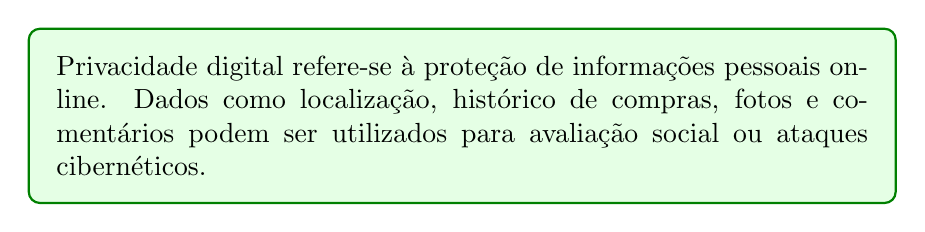
\begin{tikzpicture}
\node[rectangle, fill=green!10, rounded corners, inner sep=10pt, draw=green!50!black, thick, text width=0.85\linewidth, align=justify] {
Privacidade digital refere-se à proteção de informações pessoais online. Dados como localização, histórico de compras, fotos e comentários podem ser utilizados para avaliação social ou ataques cibernéticos.
};
\end{tikzpicture}

\vspace{3mm}

\subsection*{Cibersegurança e Proteção}

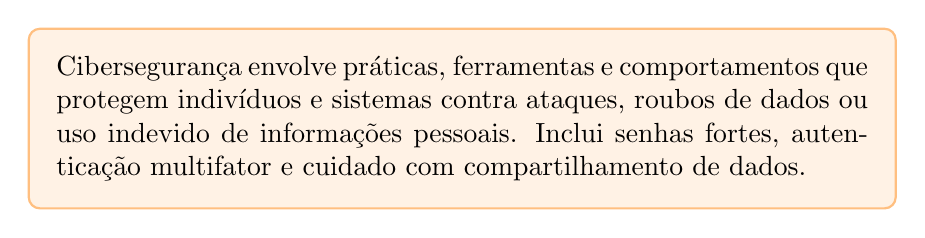
\begin{tikzpicture}
\node[rectangle, fill=orange!10, rounded corners, inner sep=10pt, draw=orange!50, thick, text width=0.85\linewidth, align=justify] {
Cibersegurança envolve práticas, ferramentas e comportamentos que protegem indivíduos e sistemas contra ataques, roubos de dados ou uso indevido de informações pessoais. Inclui senhas fortes, autenticação multifator e cuidado com compartilhamento de dados.
};
\end{tikzpicture}

\vspace{5mm}

\section*{3. Atividade Prática: Avaliação Social e Segurança}

\textbf{Cenário:} Imagine que você vive em um mundo onde cada ação online recebe uma nota que afeta diretamente suas oportunidades. Como no episódio, cada comentário, curtida ou postagem é avaliado por todos.

\begin{enumerate}[leftmargin=*]
\item Identifique três situações em que suas ações online poderiam impactar sua reputação.\\[4\baselineskip]

\item Proponha estratégias para proteger sua privacidade e dados pessoais em cada situação.\\[4\baselineskip]

\item Analise os riscos de exposição em redes sociais, apps e fóruns.\\[4\baselineskip]

\end{enumerate}


\vspace{5mm}

\section*{4. Dica de Segurança}

\begin{center}
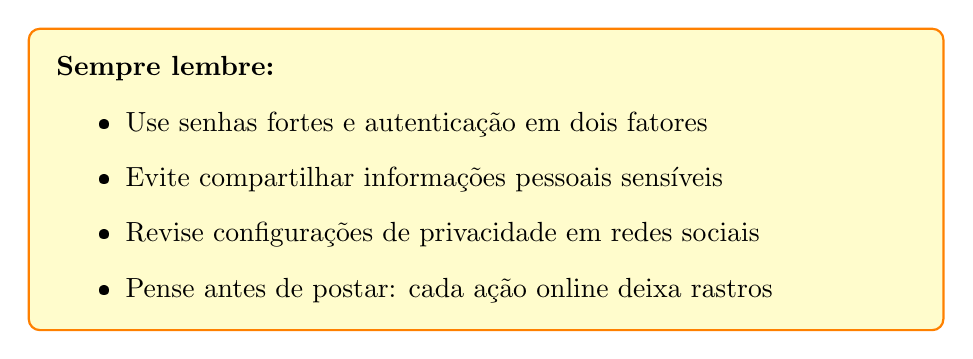
\begin{tikzpicture}
\node[rectangle, fill=yellow!20, rounded corners, inner sep=10pt, draw=orange, thick, text width=0.9\linewidth, align=justify] {
\textbf{Sempre lembre:}
\begin{itemize}
\item Use senhas fortes e autenticação em dois fatores
\item Evite compartilhar informações pessoais sensíveis
\item Revise configurações de privacidade em redes sociais
\item Pense antes de postar: cada ação online deixa rastros
\end{itemize}
};
\end{tikzpicture}
\end{center}

\section*{5. Questões de Cibersegurança}

\begin{enumerate}[leftmargin=*]

\item O que significa reputação digital?
\begin{enumerate}[label=\alph*)]
\item A pontuação que uma pessoa recebe em jogos online.
\item A percepção que outros têm sobre você baseada em suas ações online.
\item A quantidade de seguidores nas redes sociais.
\item O uso de senhas fortes.
\end{enumerate}

\item Qual prática ajuda a proteger sua privacidade online?
\begin{enumerate}[label=\alph*)]
\item Compartilhar fotos em redes públicas.
\item Usar a mesma senha para todas as contas.
\item Revisar configurações de privacidade e limitar compartilhamento de dados.
\item Postar sobre localização em tempo real.
\end{enumerate}

\item O que é autenticação em dois fatores?
\begin{enumerate}[label=\alph*)]
\item Um tipo de antivírus gratuito.
\item Um método de segurança que combina senha e um segundo fator, como código temporário.
\item Uma forma de reduzir seguidores.
\item Um filtro de rede social.
\end{enumerate}

\item Qual risco está associado ao excesso de exposição online?
\begin{enumerate}[label=\alph*)]
\item Melhora a memória do computador.
\item Aumento do risco de ataques cibernéticos e dano à reputação.
\item Diminuição do uso de senhas.
\item Maior chance de ganhar seguidores.
\end{enumerate}

\item Senhas fortes devem conter:
\begin{enumerate}[label=\alph*)]
\item Apenas letras minúsculas.
\item Apenas números.
\item Combinação de letras maiúsculas, minúsculas, números e símbolos.
\item O nome do usuário.
\end{enumerate}

\item O episódio "Odiados pela Nação" de *Black Mirror* ilustra:
\begin{enumerate}[label=\alph*)]
\item Como jogos online podem afetar a vida real.
\item O impacto da avaliação social e da exposição digital na vida pessoal.
\item Técnicas de programação.
\item Métodos de criptografia avançada.
\end{enumerate}

\item Qual comportamento ajuda a reduzir riscos em redes sociais?
\begin{enumerate}[label=\alph*)]
\item Aceitar qualquer solicitação de amizade.
\item Pensar antes de postar e revisar quem pode ver seu conteúdo.
\item Publicar tudo em contas públicas.
\item Não usar redes sociais.
\end{enumerate}

\item Qual é uma consequência de compartilhar informações pessoais sensíveis?
\begin{enumerate}[label=\alph*)]
\item Aumento da privacidade.
\item Possível uso indevido, como golpes, roubos de identidade ou dano à reputação.
\item Mais seguidores fiéis.
\item Senhas mais seguras.
\end{enumerate}

\item Cibersegurança inclui:
\begin{enumerate}[label=\alph*)]
\item Apenas instalar antivírus.
\item Práticas, ferramentas e comportamentos que protegem dados e sistemas.
\item Aumento de curtidas em redes sociais.
\item Compartilhamento irrestrito de dados.
\end{enumerate}

\item Como agir se encontrar um comentário malicioso sobre você online?
\begin{enumerate}[label=\alph*)]
\item Ignorar e apagar suas próprias contas.
\item Revidar publicamente com críticas.
\item Avaliar a situação, denunciar ou bloquear, e proteger sua privacidade.
\item Compartilhar com todos para alertar.
\end{enumerate}

\end{enumerate}


\end{multicols}

\end{document}

